\documentclass[10pt,conference,compsocconf]{IEEEtran}

\usepackage{hyperref}
\usepackage{graphicx}	% For figure environment
\usepackage{natbib}

\begin{document}
\title{Process Book}

\author{
  Rehan Mulakhel, Noemi Romano, Raja Soufi\\
  \textit{Department of Computer Science, EPFL Lausanne, Switzerland}
}

\maketitle

\begin{abstract}
A critical part of scientific discovery is the communication of research findings to peers or the general public. Mastery of the process of scientific communication improves the visibility and impact of research. While this guide is a necessary tool for learning how to write in a manner suitable for publication at a scientific venue, it is by no means sufficient, on its own, to make its reader an accomplished writer. This guide should be a starting point for further development of writing skills.
\end{abstract}

\section{Introduction}

Over human history, thousands and thousands of meteorites fell to the Earth ground; chunk of rock and metal disagreggating in the atmosphere, hitting the ground and causing sometimes vast disasters. 

The goal of this project is to visualize this fascinating phenomenon occurred over the last centuries by means of georeferenced location of the impacts recorded by the $Meteoritical$ $society$\footnote{Meteoritical society: http://www.meteoriticalsociety.org/}. In this visualization, our principal aim is to give a general overview of the spatio-temporal evolution of this natural phenomenon, emphasizing on the user experience and the exploration of the data. This visualization targets a general public who has not strong knowledge in the field. 


\section{Data}
\label{sec:data}
The data come from the NASA’s Open Data Portal and have been downloaded from Kaggle’s platform. The data were collected by The Meteoritical Society and contain information on all of the known meteorite landings. The dataset includes the following fields:

\begin{description}
\item[\texttt{name}] \ \\
  The name of the meteorite (typically a location, often modified with a number, year, composition, etc).
\item[\texttt{id}] \ \\
  The unique identifier for the meteorite.
\item[\texttt{nametype}] \ \\
  One of: -- \texttt{valid}: a typical meteorite -- \texttt{relict}: a meteorite that has been highly degraded by weather on Earth.
\item[\texttt{recclass}] \ \\
  The class of the meteorite; one of a large number of classes based on physical, chemical, and other characteristics.
\item[\texttt{mass}] \ \\
  The mass of the meteorite, in grams.
\item[\texttt{fall}] \ \\
   Whether the meteorite was seen falling, or was discovered after its impact; one of: -- Fell: the meteorite's fall was observed -- Found: the meteorite's fall was not observed.
\item[\texttt{year}] \ \\
  The year the meteorite fell, or the year it was found (depending on the value of fell).
\item[\texttt{reclat}] \ \\
  The latitude of the meteorite's landing.
\item[\texttt{reclong}] \ \\
  The longitude of the meteorite's landing.
\item[\texttt{GeoLocation}] \ \\
  The parentheses-enclose, comma-separated tuple that combines \texttt{reclat} and \texttt{reclong}.
\end{description}

Rows containing \texttt{NaN} values or presenting a year’s value smaller than $860$ and bigger than $2016$ (suggestion of the Kaggle’s description of the data) will not be considered in our visualization project. In addition, some of the entries having coordinates values equal to $0$ ---referring to meteorites found in Antarctica of which coordinates were not given--- will not be considered. 

% TODO: topojson & three

After the cleaning, we end up with a final number of $31,705$ over $45,716$ entries.

\section{Tools}
\label{sec:tools}

The visualization is displayed in a browser for usability reasons: users do not need to download anything. This forces the application to be split into a front-end and back-end.

\subsection{Front-end}

The dynamic suggestion appearing when typing a country is done with Bootstrap which is stored in a CDN.

Jquery is used to easily switch tabs in the statistics window.

% TODO: topojson & three

\subsection{Back-end}

To do.

\section{Evolution of visualization}
\label{sec:evolution_of_visualization}

The first step was to figure out which visualization could be appropriate to visualize the spatial distribution of the meteorites' impacts. A globe or a map with the georeferenced impacts as static points came to our mind, but the UX would have been limited. That's why we decided to animate the trajectory of the meteorite falls, in order to give a realistic dimension to the data. In order to enforce the realistic dimension we prioritized the 3D visualization, hence a globe has been chosen to visualize the geographical space. To give a more global point of view of the spatial distribution of this phenomena, the transition from the globe to a 2D map has been also taken into account. 

Having the coordinates of the impacts, it was crucial to get the country where the meteorites fell. Getting access to the country implies then a new category of classification, leading to a local and easier exploration of the data. The local dimension gave us new ideas for the data representation: 

\begin{itemize}
\item Visualization of the country related statistics
\item A search-bar where the user can enter the country wished
\item The interaction user-globe that allows to click over a country and see the meteorites falling for the country selected 
\item Histogram of the type of meteorite by country
\end{itemize}

A time-line was by far the easiest way to visualize the temporal dimension. In order to add an interaction to it, we decided to allow the selection of an interval of time to the user. The animation of the meteorites falls will be then performed in the interval of time selected and activated/deactivated with a start/pause button. 

Here below our first sketch of the visualization:
\iffalse
\begin{figure}[tbp]
  \centering
  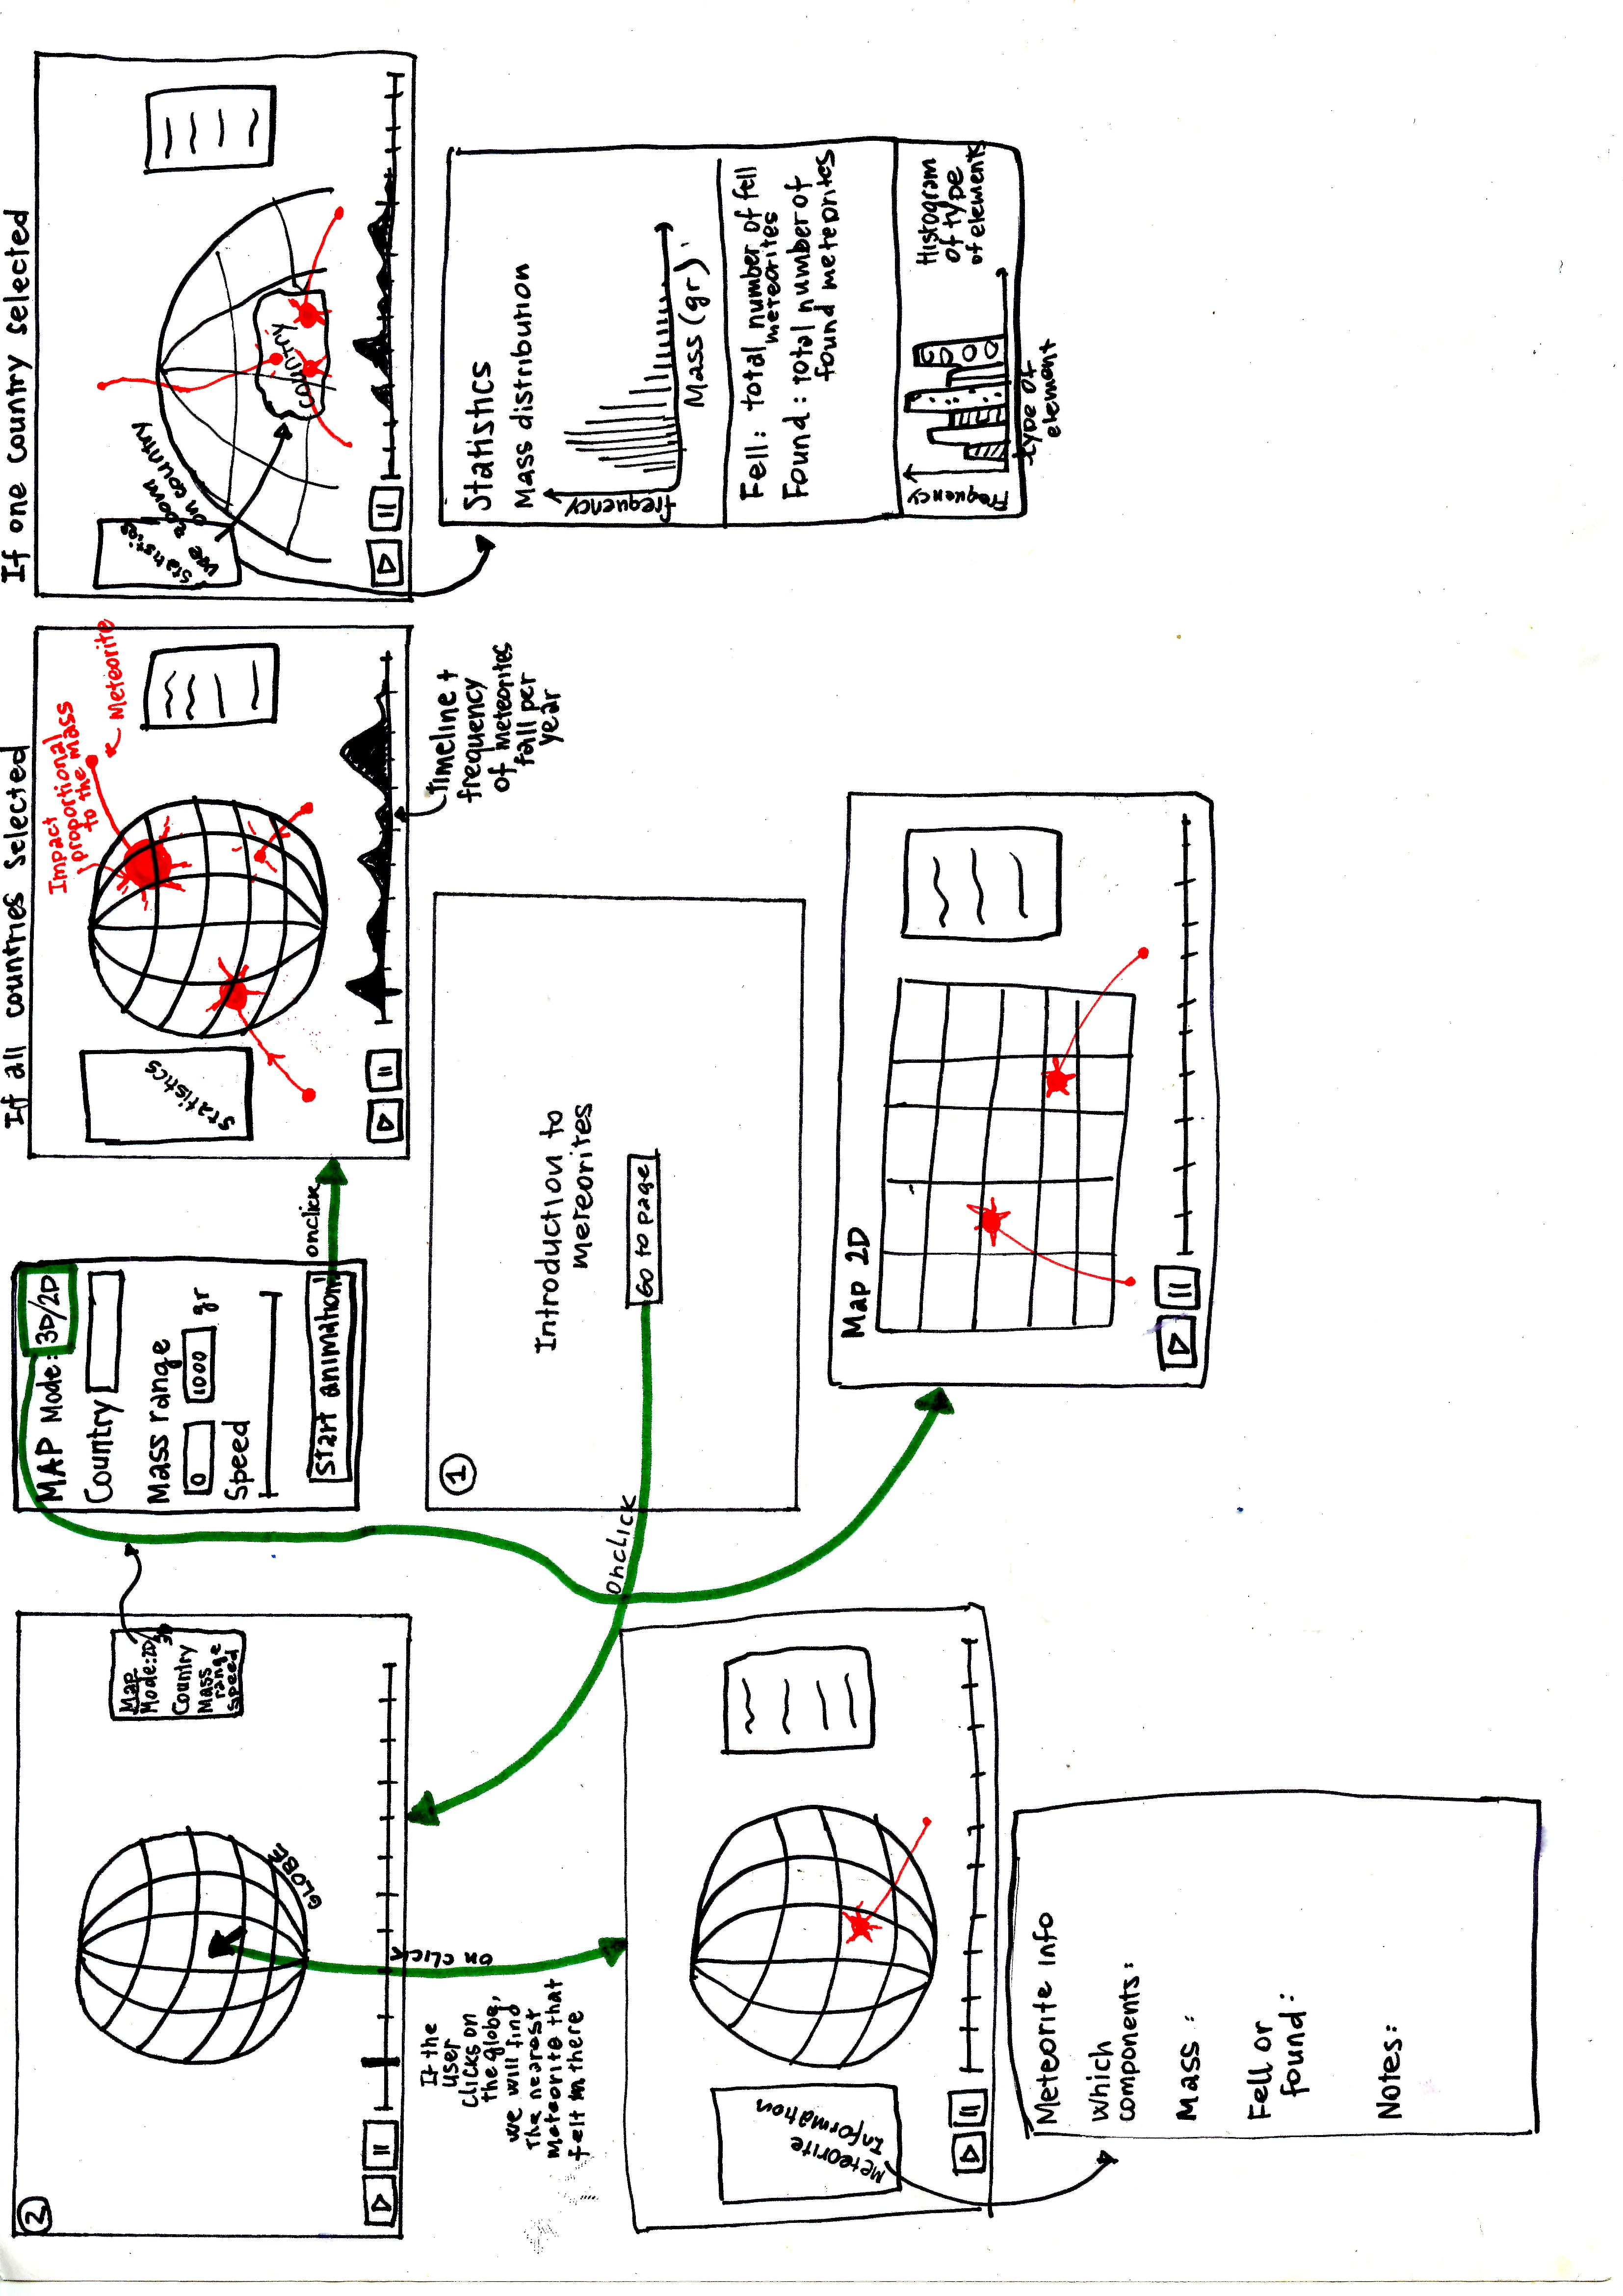
\includegraphics[width=\columnwidth]{sketch1}
  \vspace{-3mm}
  \caption{First sketch of the visualization}
  \label{fig:denoise-wavelet}
\end{figure}
\fi


\subsection{Globe}
Exploring the Mike Bostock's Blocks \cite{bostock_mike_nodate} we discovered many tutorial allowing the creation of a globe with $d3.js$ \cite{bostock_see-through_nodate,bostock_globe_nodate}.  These works are performed with the $d3.geo$ library that allows an easy way to work with geographic information and different projections.
We then created the globe, but a sticking point came up: how to visualize the meteorites' animation with $d3$? 

 
%This process has been %performed with... %openstreet map \\

 











Use examples and illustrations to clarify ideas and results. Figure~\ref{fig:denoise-wavelet}, we can see the two different situations where Fourier and wavelet basis perform well.

\section{Improvements}
\label{sec:improvements}

To do.

\section{Work split}
\label{sec:work_split}

\begin{description}
\item[Rehan Mulakhel] \ \\
  Web page centralizing links to the demo, code and process book. General design of the demo page. Brushing time line. Dynamic suggestion for the countries. Country to each meteorite based on coordinates. 
\item[Noemi Romano] \ \\
  To do.
\item[Raja Soufi] \ \\
  To do.
\end{description}




\bibliography{geometeorites}
\bibliographystyle{plain}



\end{document}
